% !Tex root = main.tex
\newpage
\section{Experiments and Results}
\label{sec:ExperimentsandResults}
In order to test the previously described \ac{TAD} approach several experiments
were performed, to find the optimal model for both the \ac{SISR} and \ac{IC}
tasks, to show the impact of the L1 ball on the model's robustness against
perturbations as well as evincing the feasibility of applying the \ac{TAD}
method in the video domain.

\begin{figure}[!htbp]
	\centering
	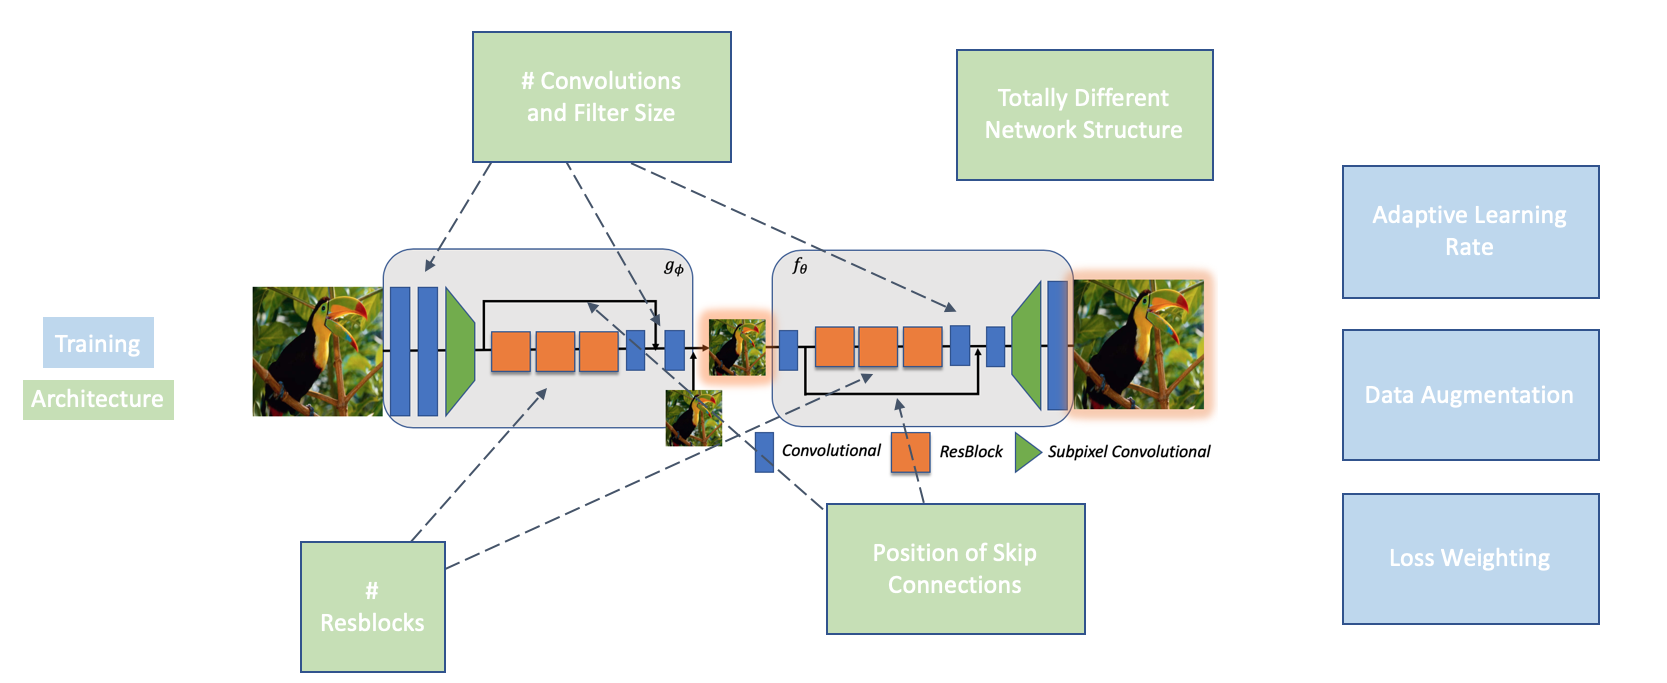
\includegraphics[width=14cm]{figures/model_adaptions}
	\caption{Model and Training adaptions during experiments in comparison
  to the baseline model by \cite{TAID}.}
  \label{fig:model_adaptions}
\end{figure}

As shown in \myfigref{fig:model_adaptions} a bunch of adjustments to the
baseline model (by \cite{TAID}) were tried for analysing the coherence between
the model complexity and its reconstruction performance. Thereby very small
architectures (6 layers) as well as comparable large architectures
(19 layers) were tested (baseline model has 10 layers), spanning
from $375.926$ to $1.299.126$ parameters. Since the model already is quite
shallow the removal of each layer had an impact on the resulting performance,
therefore especially the number of \textit{Resblocks} (two convolutional layers
and ReLU) has a huge impact on the reconstruction accuracy. Next to adaptions
to the baseline architecture completly new architectures have been tested, such
as networks without any residual pass (so no Resblocks) but convolutional layers
with either constant or varying (first increasing then decreasing) number of
filters (up to 256) have been used.
\newline
Next to several architectures the baseline model was improved by advancing the
training procedure. Next to enhancing the loss function as discussed in
\mysecref{sec:Approach_LF} instead of a constant an linearly annealing learning
rate was used, starting at $4*10^{-4}$ and annealing by factor $\gamma = 0.25$
after $20$, $100$ and again after $200$ training epochs. Adam optimizer was used
with $\beta = (0.9, 0.999)$, $\epsilon_{ADAM} = 10^{-8}$, gradient clipping and
zero weight decay.
\newline
To guarantee comparability to other super-resolution and colorization paper
in the image domain the model was trained using the DIV2K training dataset
(\cite{DIV2K}), while validated on the SET5 (\cite{SET5}), SET14 (\cite{SET14}),
BSDS100 (\cite{BSDS100}), URBAN100 (\cite{URBAN100}) and VDIV2K (\cite{DIV2K})
dataset. For similar reason for the video domain the model was pretrained using
DIV2K, actually trained on video clips from CDVL Database (Ntiaspen) and
validated on the widely known Vid4 dataset (Calendar, Foliage, Walk, City).
For improving generalization capabilities of the model and avoid overfitting
the image training data were also augmented (rotated, mirrored).
\newline
Similiarly, as widely used in the field of image reconstruction as a performance
measurement the \ac{PSNR} will be used.
\newline
A complete list of the most important testing configurations and their results
as well as a list of architectures can be found in the appendix.

\subsection{Impact of L1 Ball}
\label{sec:Experiments_EPS_BALL}
As already seen in \mychapterref{sec:Approach} introducing an $\epsilon$-ball
to the loss term pervents the model from overfitting on the low-dimensional
image, $X_{SLR} = X_{GD}$ (i.e. trivial solution $g_\theta = 0$ in the
beginning of the training).\footnote{As discussed in \mychapterref{sec:Approach}
the training is splitted into two parts, first learning only the difference
between the guidance image and a more optimal representation and later
learning the low-dimensional representation independent from the guidance
image.} However, the main contribution of the $\epsilon$-ball consists in the
increasing robustness against perturbations of $X_{SLR}$, which are modeled
as white Gaussian noise with standard deviation $\sigma$ within this project.
While a model trained with $\epsilon = 0$ is highly vulnerable to perturbations,
dropping \ac{PSNR} by $42 \%$ by adding noise with $\sigma = 0.11$ ($X_{SLR} \in
[0,1]^n$), a model trained with $\epsilon = 10$ is more stable dropping only
about $10 \%$ in the same scenario (scale = 4, dataset = SET14).

\begin{figure}[!htbp]
	\centering
	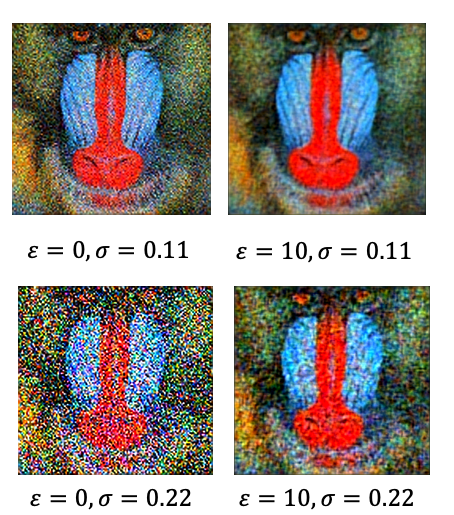
\includegraphics[width=8cm]{figures/epsball_qualitative_comp}
	\caption{Qualitative comparison between the impact of perturbation on a
  model trained without and with $\epsilon$-ball (scale = 4, dataset = SET14).}
  \label{fig:epsball_qualitative_comp}
\end{figure}

In the following experiment the same model (AETAD)\footnote{An overview over
all model architectures can be found in the appendix.} was trained with different
radii of the $\epsilon$-ball. It turns out that the right choice of $\epsilon$
is a trade-off between the reconstruction performance and robustness aginst
perturbations, comp. \myfigref{fig:epsball_perturbation}.

\begin{figure}[!htbp]
	\centering
	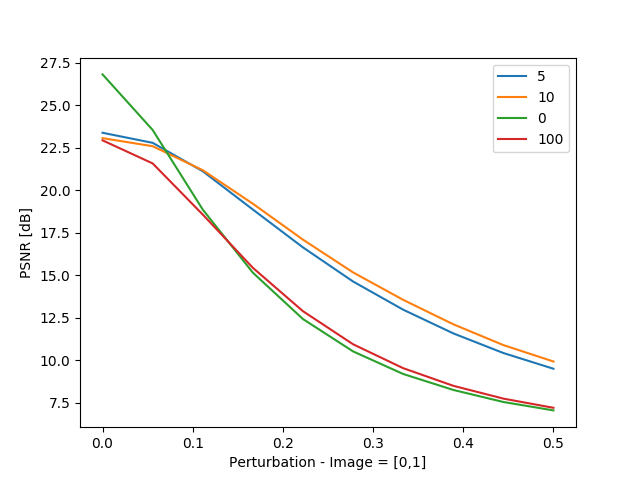
\includegraphics[width=10cm]{figures/epsball_perturbation}
	\caption{Reconstruction performance over several values of $\epsilon$
  and $\sigma$ (scale = 4).}
  \label{fig:epsball_perturbation}
\end{figure}

Also an increasing
$\epsilon$ improves the convergence rate during training, as shown in
\myfigref{fig:epsball_loss}, the model otherwise first overfits to $X_{GD}$
and then eventually finds a more optimal trade-off between fitting the
low- and high-dimensional image (with increasing $\frac{\alpha}{\beta}$ ratio).
However, as \myfigref{fig:epsball_perturbation} the radius of the $\epsilon$-ball
around $X_{GD}$ cannot be choosen infinitely large, since the overall performance
worsens as the impact of the guidance image on the model convergence decreases
(e.g. $\epsilon = 100$ in \myfigref{fig:epsball_perturbation}). Overall an
radius $\epsilon = 20$ was found to be the best performing configuration.
Although described for the \ac{SISR} problem here the described impact of
the $\epsilon$-ball is similar over all other problems, which omitted here
for the matter of compactness of this report.

\begin{figure}[!htbp]
	\centering
	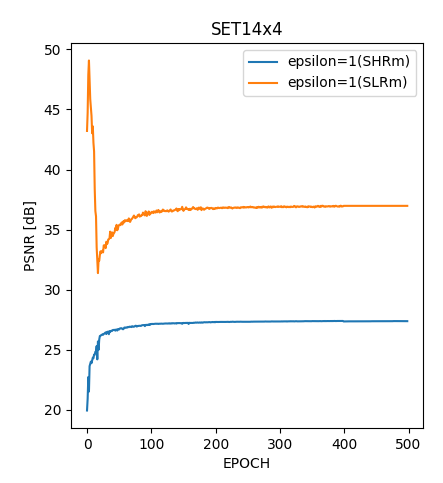
\includegraphics[width=6cm]{figures/epsball_loss_1_set14}
  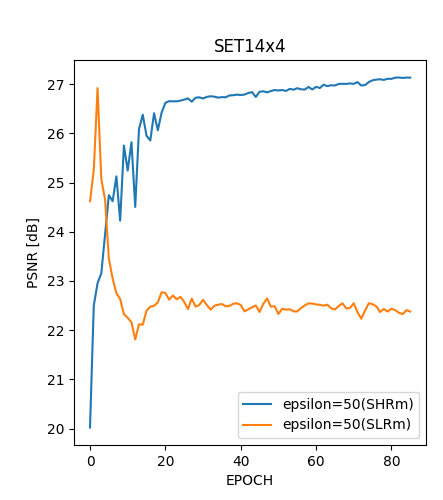
\includegraphics[width=6cm]{figures/epsball_loss_50_set14}
	\caption{Closeness between $X_{SLR}$ and guidance image (blue) and $X_{SHR}$
  and groudtruth image (orange) for different values of $\epsilon$ (left:
  $\epsilon = 1$, right $\epsilon = 50$).}
  \label{fig:epsball_loss}
\end{figure}

\subsection{Single-Image Super-Resolution}
\label{sec:Experiments_SISR}
Next to improving the robustness of the \ac{TAD} model several improvements
were made on both the way of training as well as on the architecture itself.
\myfigref{fig:psnr_complexty_sisr} shows the correlation on both the SET5
and the SET14 dataset for different architectures which were trained using the
same parameters (learning parameters as described above, $\epsilon = 10$) for
the sake of a comparability.

\begin{figure}[!htbp]
	\centering
	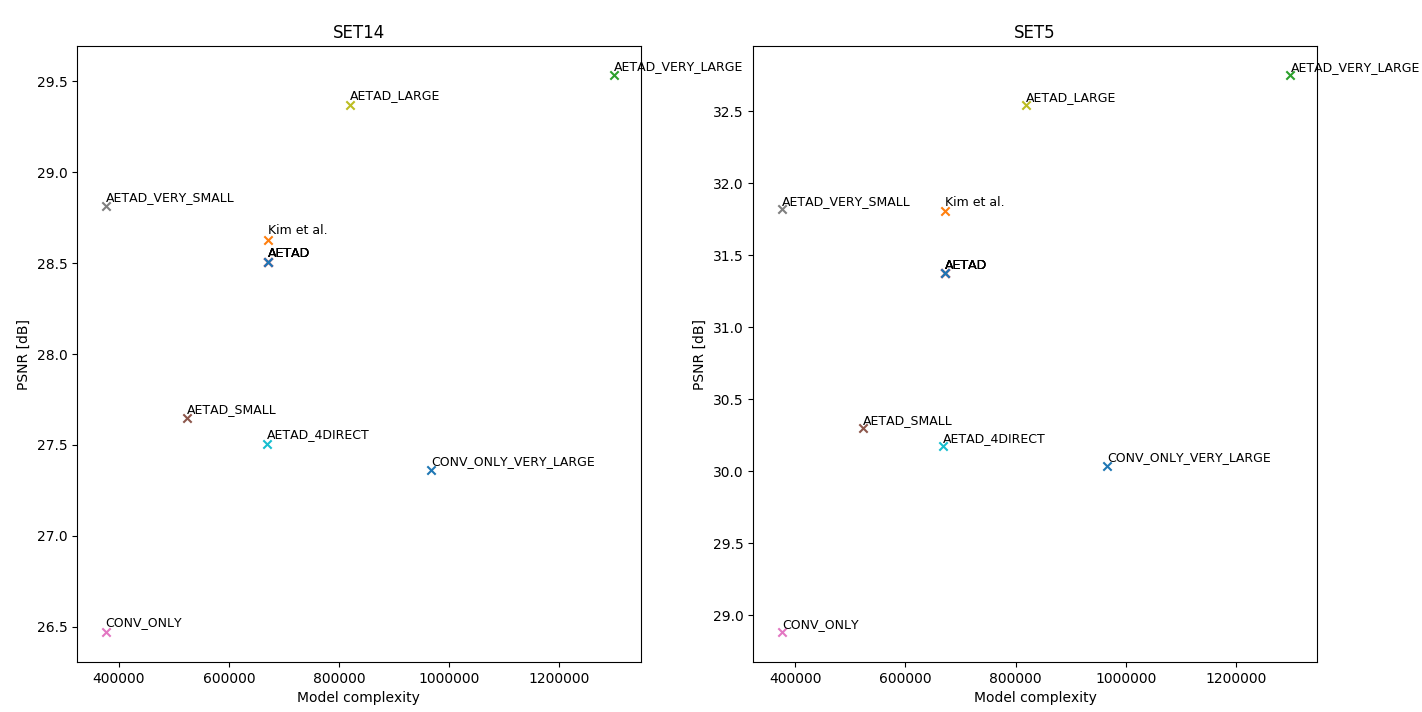
\includegraphics[width=14cm]{figures/psnr_complexty_sisr}
	\caption{Model complexity vs reconstruction performance for \ac{SISR}
	problem (scale = 4, dataset = SET14 and SET5).}
  \label{fig:psnr_complexty_sisr}
\end{figure}

Several conclusion can be drawn from \myfigref{fig:psnr_complexty_sisr}, which
could be confirmed also for the other validation datasets used:

\begin{itemize}
\item The \textit{Resblocks} have a large impact on the models performance,
purely convolutional models with neither a skip connection nor a ReLU layer
(as occurring in \textit{Resblocks}), such as the models \textit{conv\_only} or
\textit{conv\_only\_very\_large}, have an overall worse reconstruction
performance with a similar number of parameters.
\item In a direct comparison the model \textit{aetad\_direct4} performs worse
than the iteratively scaling structured, but otherwise equivalent model
\textit{aetad}.
\item In both displayed validation datasets the reconstruction performance
stagnates with increasing number of parameters, as the difference in \ac{PSNR}
between the \textit{aetad\_large} and the \textit{aetad\_very\_large}
model does not improve much anymore.
\end{itemize}

While more complex architectures than the baseline (\textit{Kim et al.}-model)
do not gain a lot of accuracy, for less complex models with similar architecture
there is a large drop in accurcy. Therefore, the baseline architecture already
is very reasonable.

\begin{enumerate}
\item different scales (maybe large scales as well)
\item performance on other non-trained scales
\item final model for other scales and other datasets
\end{enumerate}

\subsection{Image Colorization}
\label{sec:Experiments_IC}

\begin{figure}[!htbp]
	\centering
	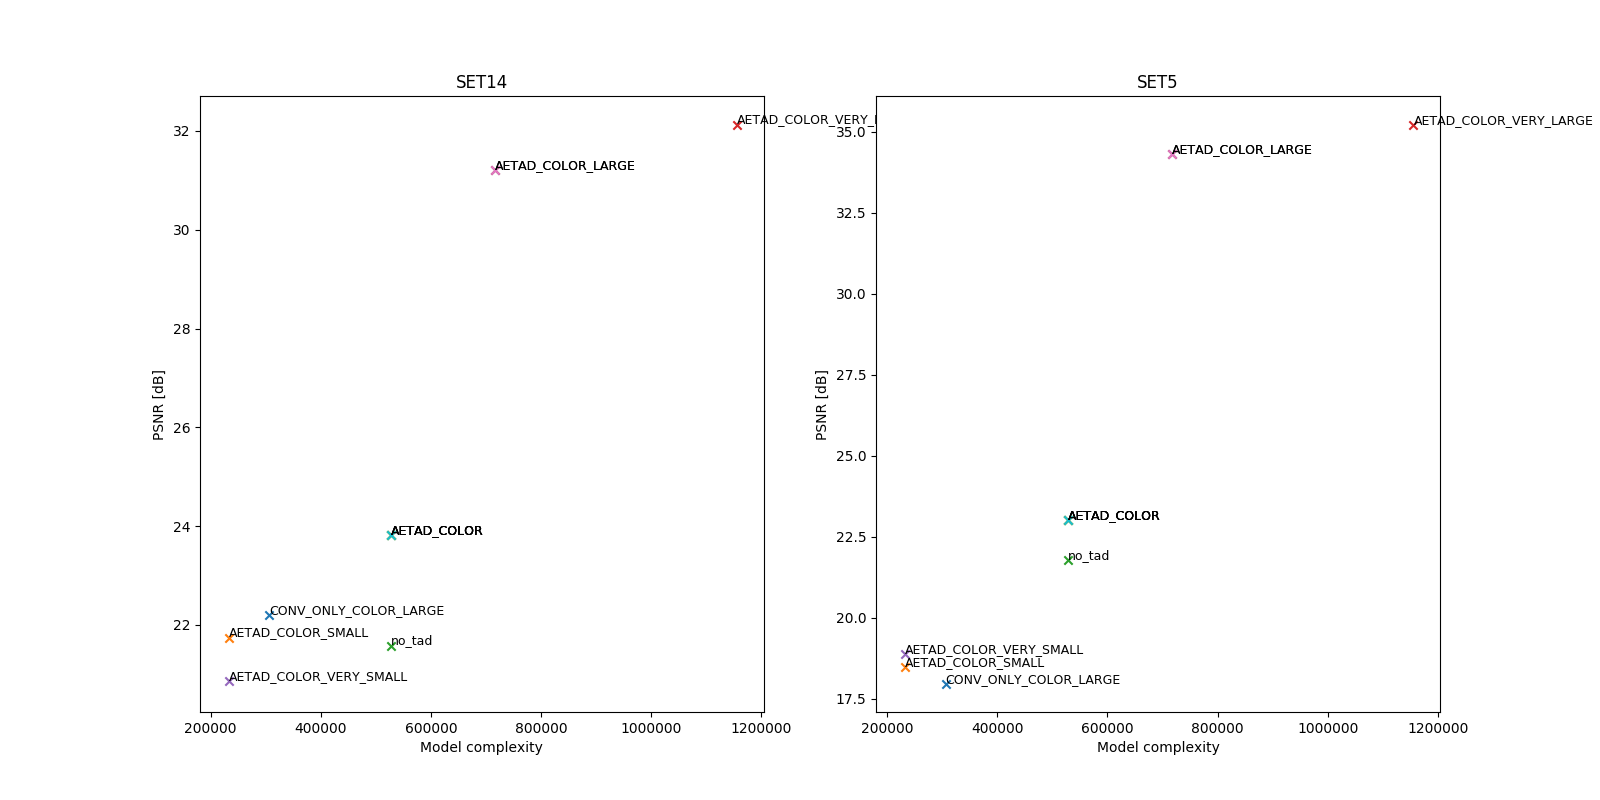
\includegraphics[width=14cm]{figures/psnr_complexity_ic}
	\caption{Model complexity vs reconstruction performance for \ac{IC}
	problem (dataset = SET14 and SET5).}
  \label{fig:psnr_complexity_ic}
\end{figure}

\subsection{Video Super-Resolution}
\label{sec:Experiments_VSR}

\begin{enumerate}
\item super-large scale for videos
\end{enumerate}

\subsection{Qualitative Improvements}
\label{sec:Experiments_QI}



\begin{enumerate}
\item gummibear image (TAD learns to downscale an image task-aware and thereby
can store information that are lost by simple downscaling (e.g. bilinear
interpolation, averaging colors). Therefore, possibly even image can restored
that are impossible to restore  using classic approaches, like exactly
similar gummibears.)
\end{enumerate}

% Describe the evaluation you did in a way, such that an independent researcher can repeat it. Cover the following questions:
% \begin{itemize}
%  \item \textit{What is the experimental setup and methodology?} Describe the setting of the experiments and give all the parameters in detail which you have used. Give a detailed account of how the experiment was conducted.
%  \item \textit{What are your results?} In this section, a \emph{clear description} of the results is given. If you produced lots of data, include only representative data here and put all results into the appendix.
% \end{itemize}
